\documentclass[11pt,a4paper,twoside]{report}
\usepackage[utf8]{inputenc}
\usepackage[portuguese]{babel}
\usepackage[T1]{fontenc}
\usepackage{fancyhdr}
\usepackage{amsmath}
\usepackage{amsfonts}
\usepackage{amssymb}
\usepackage{makeidx}
\usepackage{graphicx}
\usepackage{lmodern}
\usepackage{wrapfig}
%\usepackage{color}
\usepackage{color,colortbl,multirow}
\usepackage{multirow}
\usepackage[table]{xcolor}
\definecolor{lightgray}{gray}{0.9}
\usepackage{float}
\usepackage{fourier}
\usepackage[left=2cm,right=2cm,top=2cm,bottom=2cm]{geometry}
\author{Bartolomeu J. Ubisse}
\pagestyle{fancy}
\renewcommand{\headrulewidth}{0pt}
\renewcommand{\footrulewidth}{1pt}
\fancyfoot[L]{ | UEM - 2017}
\fancyfoot[c]{}
\fancyfoot[r]{\thepage}
\begin{document}


\begin{figure}[htb]

\centering

\includegraphics[scale=1]{UEM-logotipo}
\end{figure}
\centering
{ \Large Universidade Eduardo Mondlane}\\[0.3cm] 
\large Faculdade de Ci\^encias\\[0.2cm]
 \large Departamento de F\'isica\\[0.5cm]

%\textsc{Electr\^onica B\'asica} \\[1cm]
\begin{flushleft}
\tt Teste 2 - E. Anal\'ogica\hspace{0.25cm} |Data:$01/06/2017$\hspace{0.25cm}|Hora:$19:10-21:10$ hrs.\\
\hrulefill
 \begin{table}[htb]
\centering
\begin{tabular}{p{16.55cm}}
\hline
\cellcolor[gray]{0.95}
Responda atentamente as perguntas que lhe s\~ao colocadas e mostre todos os passos necess\'arios.\\

 \hline
\end{tabular}
\end{table}
\end{flushleft}

\begin{enumerate}
\item Uma das diferen\c cas entre TBJs e JFETs reside no mecanismo de controle de correntes de saida em cada um deles. Explique como \'e que isso se procede.[\textit{$3.5$ Valores}]
\item Explique o que entende por tens\~ao limiar num NMOS de tipo enriquecimento.[\textit{$3.5$ Valores}]
\item Explique o que entende por corrente de manuten\c c\~ao (\textit{holding current}) num SCR.[$3.0$ Valores]
\item Detemine o ganho de tens\~ao do amplificador da fig.\ref{f2} considerando que $V_T=26$mV.[\textit{$6.0$ Valores}]
\item Determine $R_D$ e $R_S$ do circu\'ito da fig.\ref{a} sabendo que  $I_D=0.4$mA, $V_{th}=2$V, $W/L=40$ e $\mu_n cox =0.02mA/V^{2}$.[\textit{$4.0$ Valores}]
\end{enumerate}
  \noindent
\begin{minipage}[c]{5cm}
 \begin{figure}[H]
\centering
\includegraphics[scale=0.7]{test2tbj}
\caption{}
\label{f2}
\end{figure}
\end{minipage}\hfill
\begin{minipage}[c]{9cm}
\begin{figure}[H]
\centering
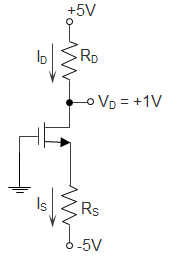
\includegraphics[scale=0.7]{MOSFET1}
\caption{}
\label{a}
\end{figure}
\end{minipage}



\vspace{1.5cm}

\huge{Bom Trabalho !}




\end{document}